\documentclass{standalone}
\usepackage{tikz}
\usetikzlibrary{patterns, positioning}


\begin{document}
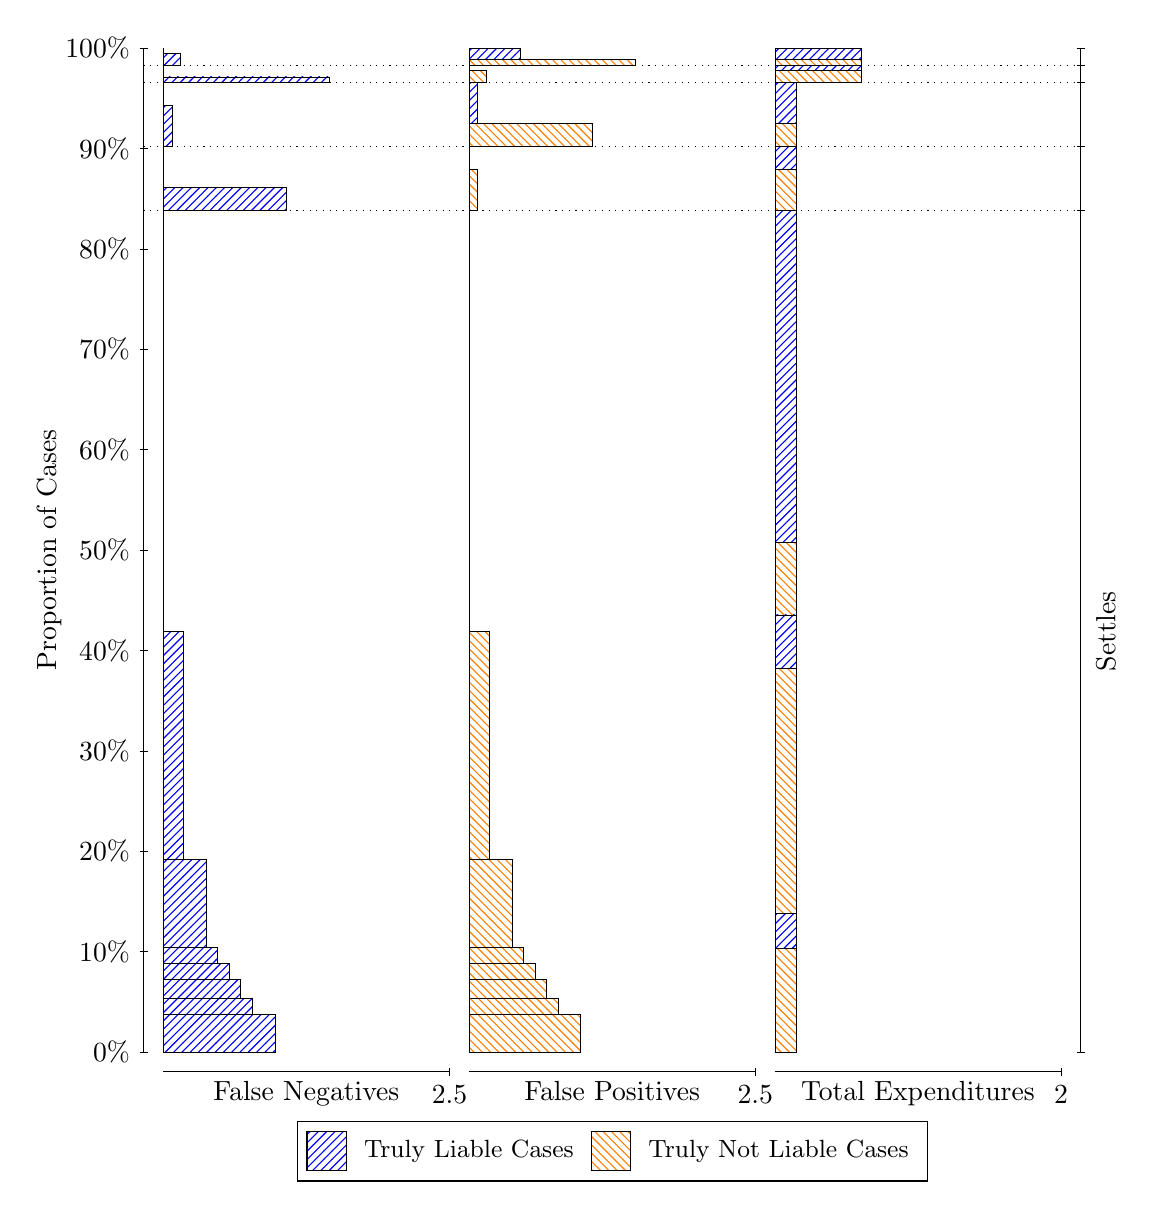
\begin{tikzpicture}
\draw[black, very thin] (1.5,1.75) -- (1.5,14.5);
\node[rotate=90, text=black, anchor=center] at (0.3, 8.125) {Proportion of Cases};
\draw[black, very thin] (1.45,1.75) -- (1.55,1.75);
\node[text=black, anchor=east] at (1.45, 1.75) {0\%};
\draw[black, very thin] (1.45,3.025) -- (1.55,3.025);
\node[text=black, anchor=east] at (1.45, 3.025) {10\%};
\draw[black, very thin] (1.45,4.3) -- (1.55,4.3);
\node[text=black, anchor=east] at (1.45, 4.3) {20\%};
\draw[black, very thin] (1.45,5.575) -- (1.55,5.575);
\node[text=black, anchor=east] at (1.45, 5.575) {30\%};
\draw[black, very thin] (1.45,6.85) -- (1.55,6.85);
\node[text=black, anchor=east] at (1.45, 6.85) {40\%};
\draw[black, very thin] (1.45,8.125) -- (1.55,8.125);
\node[text=black, anchor=east] at (1.45, 8.125) {50\%};
\draw[black, very thin] (1.45,9.4) -- (1.55,9.4);
\node[text=black, anchor=east] at (1.45, 9.4) {60\%};
\draw[black, very thin] (1.45,10.675) -- (1.55,10.675);
\node[text=black, anchor=east] at (1.45, 10.675) {70\%};
\draw[black, very thin] (1.45,11.95) -- (1.55,11.95);
\node[text=black, anchor=east] at (1.45, 11.95) {80\%};
\draw[black, very thin] (1.45,13.225) -- (1.55,13.225);
\node[text=black, anchor=east] at (1.45, 13.225) {90\%};
\draw[black, very thin] (1.45,14.5) -- (1.55,14.5);
\node[text=black, anchor=east] at (1.45, 14.5) {100\%};

\draw[black, very thin] (13.4,1.75) -- (13.4,14.5);
\draw[black, very thin] (13.35,1.75) -- (13.45,1.75);
\node[anchor=west] at (13.35, 1.75) {};
\draw[black, very thin] (13.35,12.437) -- (13.45,12.437);
\node[anchor=west] at (13.35, 12.437) {};
\draw[black, very thin] (13.35,13.251) -- (13.45,13.251);
\node[anchor=west] at (13.35, 13.251) {};
\draw[black, very thin] (13.35,14.064) -- (13.45,14.064);
\node[anchor=west] at (13.35, 14.064) {};
\draw[black, very thin] (13.35,14.282) -- (13.45,14.282);
\node[anchor=west] at (13.35, 14.282) {};
\draw[black, very thin] (13.35,14.5) -- (13.45,14.5);
\node[anchor=west] at (13.35, 14.5) {};

\draw[black, very thin, pattern color=blue, pattern=north east lines] (1.75,1.75) rectangle (3.167,2.2264);
\draw[black, very thin, pattern color=blue, pattern=north east lines] (1.75,2.2264) rectangle (2.8763,2.4332);
\draw[black, very thin, pattern color=blue, pattern=north east lines] (1.75,2.4332) rectangle (2.731,2.6736);
\draw[black, very thin, pattern color=blue, pattern=north east lines] (1.75,2.6736) rectangle (2.5857,2.8796);
\draw[black, very thin, pattern color=blue, pattern=north east lines] (1.75,2.8796) rectangle (2.4403,3.079);
\draw[black, very thin, pattern color=blue, pattern=north east lines] (1.75,3.079) rectangle (2.295,4.1917);
\draw[black, very thin, pattern color=blue, pattern=north east lines] (1.75,4.1917) rectangle (2.0043,7.0935);
\draw[black, very thin, pattern color=orange, pattern=north west lines] (1.75,7.0935) rectangle (1.75,12.437);
\draw[black, very thin, pattern color=blue, pattern=north east lines] (1.75,12.437) rectangle (3.3123,12.727);
\draw[black, very thin, pattern color=orange, pattern=north west lines] (1.75,12.727) rectangle (1.75,13.251);
\draw[black, very thin, pattern color=blue, pattern=north east lines] (1.75,13.251) rectangle (1.859,13.774);
\draw[black, very thin, pattern color=orange, pattern=north west lines] (1.75,13.774) rectangle (1.75,14.064);
\draw[black, very thin, pattern color=blue, pattern=north east lines] (1.75,14.064) rectangle (3.8573,14.133);
\draw[black, very thin, pattern color=orange, pattern=north west lines] (1.75,14.133) rectangle (1.75,14.282);
\draw[black, very thin, pattern color=blue, pattern=north east lines] (1.75,14.282) rectangle (1.968,14.431);
\draw[black, very thin, pattern color=orange, pattern=north west lines] (1.75,14.431) rectangle (1.75,14.5);
\draw[black, very thin, pattern color=orange, pattern=north west lines] (5.6333,1.75) rectangle (7.0503,2.2264);
\draw[black, very thin, pattern color=orange, pattern=north west lines] (5.6333,2.2264) rectangle (6.7597,2.4332);
\draw[black, very thin, pattern color=orange, pattern=north west lines] (5.6333,2.4332) rectangle (6.6143,2.6736);
\draw[black, very thin, pattern color=orange, pattern=north west lines] (5.6333,2.6736) rectangle (6.469,2.8796);
\draw[black, very thin, pattern color=orange, pattern=north west lines] (5.6333,2.8796) rectangle (6.3237,3.0791);
\draw[black, very thin, pattern color=orange, pattern=north west lines] (5.6333,3.0791) rectangle (6.1783,4.1917);
\draw[black, very thin, pattern color=orange, pattern=north west lines] (5.6333,4.1917) rectangle (5.8877,7.0936);
\draw[black, very thin, pattern color=blue, pattern=north east lines] (5.6333,7.0936) rectangle (5.6333,12.437);
\draw[black, very thin, pattern color=orange, pattern=north west lines] (5.6333,12.437) rectangle (5.7423,12.961);
\draw[black, very thin, pattern color=blue, pattern=north east lines] (5.6333,12.961) rectangle (5.6333,13.251);
\draw[black, very thin, pattern color=orange, pattern=north west lines] (5.6333,13.251) rectangle (7.1957,13.54);
\draw[black, very thin, pattern color=blue, pattern=north east lines] (5.6333,13.54) rectangle (5.7423,14.064);
\draw[black, very thin, pattern color=orange, pattern=north west lines] (5.6333,14.064) rectangle (5.8513,14.213);
\draw[black, very thin, pattern color=blue, pattern=north east lines] (5.6333,14.213) rectangle (5.6333,14.282);
\draw[black, very thin, pattern color=orange, pattern=north west lines] (5.6333,14.282) rectangle (7.7407,14.351);
\draw[black, very thin, pattern color=blue, pattern=north east lines] (5.6333,14.351) rectangle (6.2873,14.5);
\draw[black, very thin, pattern color=orange, pattern=north west lines] (9.5167,1.75) rectangle (9.7892,3.0621);
\draw[black, very thin, pattern color=blue, pattern=north east lines] (9.5167,3.0621) rectangle (9.7892,3.5093);
\draw[black, very thin, pattern color=orange, pattern=north west lines] (9.5167,3.5093) rectangle (9.7892,6.6172);
\draw[black, very thin, pattern color=blue, pattern=north east lines] (9.5167,6.6172) rectangle (9.7892,7.2996);
\draw[black, very thin, pattern color=orange, pattern=north west lines] (9.5167,7.2996) rectangle (9.7892,8.2232);
\draw[black, very thin, pattern color=blue, pattern=north east lines] (9.5167,8.2232) rectangle (9.7892,12.437);
\draw[black, very thin, pattern color=orange, pattern=north west lines] (9.5167,12.437) rectangle (9.7892,12.961);
\draw[black, very thin, pattern color=blue, pattern=north east lines] (9.5167,12.961) rectangle (9.7892,13.251);
\draw[black, very thin, pattern color=orange, pattern=north west lines] (9.5167,13.251) rectangle (9.7892,13.54);
\draw[black, very thin, pattern color=blue, pattern=north east lines] (9.5167,13.54) rectangle (9.7892,14.064);
\draw[black, very thin, pattern color=orange, pattern=north west lines] (9.5167,14.064) rectangle (10.607,14.213);
\draw[black, very thin, pattern color=blue, pattern=north east lines] (9.5167,14.213) rectangle (10.607,14.282);
\draw[black, very thin, pattern color=orange, pattern=north west lines] (9.5167,14.282) rectangle (10.607,14.351);
\draw[black, very thin, pattern color=blue, pattern=north east lines] (9.5167,14.351) rectangle (10.607,14.5);
\draw[black, dotted] (1.5,12.437) -- (13.4,12.437);
\draw[black, dotted] (1.5,13.251) -- (13.4,13.251);
\draw[black, dotted] (1.5,14.064) -- (13.4,14.064);
\draw[black, dotted] (1.5,14.282) -- (13.4,14.282);
\draw[black, very thin] (1.75,1.5) -- (5.3833,1.5);
\node[text=black, anchor=north] at (3.5667, 1.5) {False Negatives};
\draw[black, very thin] (5.3833,1.45) -- (5.3833,1.55);
\node[text=black, anchor=north] at (5.3833, 1.45) {2.5};

\draw[black, very thin] (5.6333,1.5) -- (9.2667,1.5);
\node[text=black, anchor=north] at (7.45, 1.5) {False Positives};
\draw[black, very thin] (9.2667,1.45) -- (9.2667,1.55);
\node[text=black, anchor=north] at (9.2667, 1.45) {2.5};

\draw[black, very thin] (9.5167,1.5) -- (13.15,1.5);
\node[text=black, anchor=north] at (11.333, 1.5) {Total Expenditures};
\draw[black, very thin] (13.15,1.45) -- (13.15,1.55);
\node[text=black, anchor=north] at (13.15, 1.45) {2};

\node[text=black, centered, rotate=90] at (13.72, 7.0936) {Settles};





\draw (7.449999999999999,1.5) node[draw=none] (baseCoordinate) {};
\begin{scope}[align=center]
        \matrix[scale=0.5, draw=black, below=0.5cm of baseCoordinate, nodes={draw}, column sep=0.1cm]{
            \node[rectangle, draw, minimum width=0.5cm, minimum height=0.5cm, pattern color=blue, pattern=north east lines] {}; &
            \node[draw=none, font=\small, text=black] (B) {Truly Liable Cases}; &
            \node[rectangle, draw, minimum width=0.5cm, minimum height=0.5cm, pattern color=orange, pattern=north west lines] {}; &
            \node[draw=none, font=\small, text=black] (B) {Truly Not Liable Cases}; \\
            };
\end{scope}

\end{tikzpicture}
\end{document}